\documentclass{article}
% translate with >> pdflatex -shell-escape <file>

% This file is used as unit test for pgfplots, copyright by Christian Feuersaenger.
% 
% See
%   http://pgfplots.sourceforge.net/pgfplots.pdf
% for pgfplots.
%
% Any required input files (for <plot table> or <plot file> or the table package) can be downloaded
% at
% http://www.ctan.org/tex-archive/graphics/pgf/contrib/pgfplots/doc/latex/
% and
% http://www.ctan.org/tex-archive/graphics/pgf/contrib/pgfplots/doc/latex/plotdata/

\usepackage{pgfplots}
\pgfplotsset{compat=1.3}

\pagestyle{empty}

\begin{document}
	\pgfplotsset{
		clip=false,
		xlabel=$x$ label,
		ylabel=$y$ label,
		zlabel=$z$ label,
		every 3d description/.append style={
			ticklabel style={draw=red},
			label style={draw=red},
			xlabel style={name=xlabel},
			ylabel style={name=ylabel},
			zlabel style={name=zlabel},
		},
		extra description/.add code={%
			\draw[blue,thick,->] (xticklabel cs:0,0) -- (xticklabel cs:1,0);
			\draw[blue,thick,->] (yticklabel cs:0,0) -- (yticklabel cs:1,0);
			\ifpgfplotsthreedim
			\draw[blue,thick,->] (zticklabel cs:0,0) -- (zticklabel cs:1,0);
			\fi
			%
			\draw[red,thick,->] (xticklabel cs:0.5,0pt) -- (xticklabel cs:0.5,50pt);
			%
			\fill[green] (xlabel.near xticklabel*) circle (2pt);
			\fill[green] (ylabel.near yticklabel*) circle (2pt);
			\ifpgfplotsthreedim
			\fill[green] (zlabel.near zticklabel*) circle (2pt);
			\fi
			%
			\fill[orange] (xlabel.near xticklabel) circle (2pt);
			\fill[orange] (ylabel.near yticklabel) circle (2pt);
			\ifpgfplotsthreedim
			\fill[orange] (zlabel.near zticklabel) circle (2pt);
			\fi
			%
		},
	}
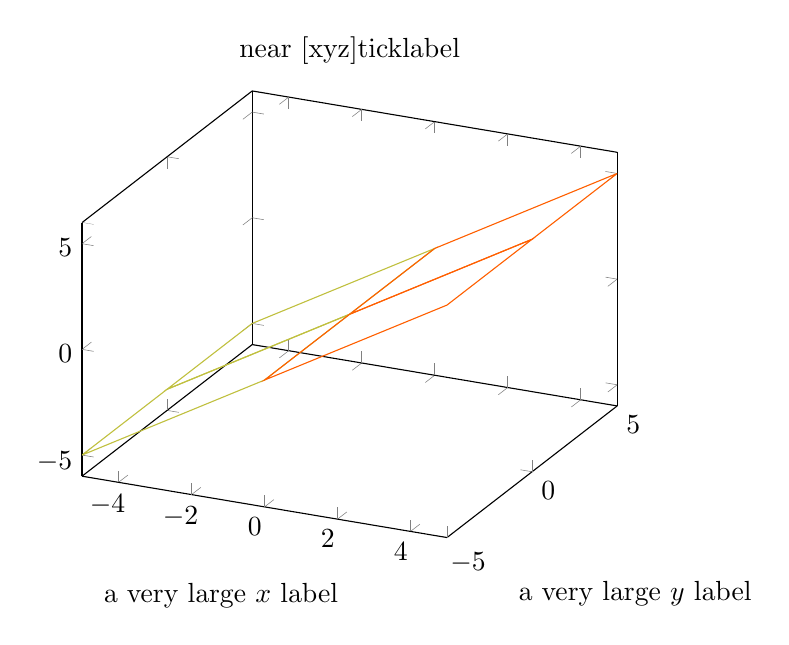
\begin{tikzpicture}
		\begin{axis}[
			title={near [xyz]ticklabel},
			xlabel=a very large $x$ label,
			ylabel=a very large $y$ label,
%every axis z label/.style={at={(ticklabel cs:0.5)},anchor=near ticklabel,name=zlabel},
		]
		
		\addplot3[mesh,samples=3] {x};
		\end{axis}
	\end{tikzpicture}
\end{document}
